\chapter{Nervous system anatomy and physiology}


\begin{description}
    \item[Central nervous system] Brain and spinal cord.
    \item[Peripheral nervous system] Nerves that branch off from the brain and the spine.
\end{description}

\section{Individual cells}

% A nervous system has two types of cells:
% \begin{descriptionlist}
%     \item[Neurons/nerve cells] 
%     \item[Glia cells/neuroglia] 
% \end{descriptionlist}


\subsection{Glia cells / Neuroglia}
\marginnote{Glia cells/Neuroglia}
Cells that support neurons.
There are 2 to 10 times more glia cells than neurons.\\

\begin{minipage}{0.89\textwidth}
    \begin{descriptionlist}
        \item[Microglia] \marginnote{Microglia}
            Immune system cells located in the central nervous system.
            They intervene in response to toxic agents or to clear dead cells.
            \begin{itemize}
                \item Responsible for antigen presentation (determine the type of external agent).
                \item Become phagocytes (cells that ingest harmful agents) during injuries, infections, or degenerative diseases.
            \end{itemize}
    
            \begin{remark}
                In patients affected by Alzheimer's disease, microglia may become hyperactive and damage neurons.
            \end{remark}
    \end{descriptionlist}
\end{minipage}
\begin{minipage}{0.1\textwidth}
    \centering
    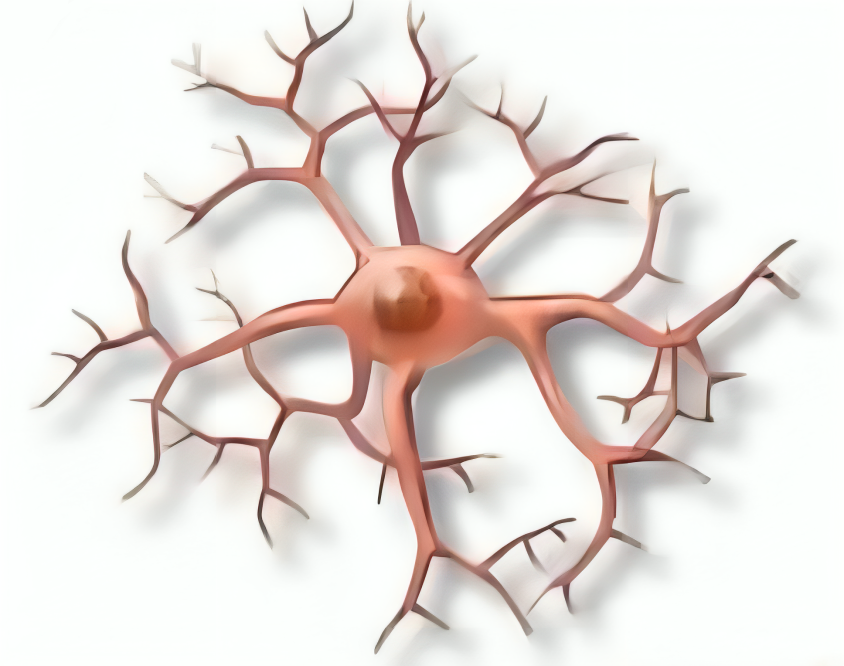
\includegraphics[width=\textwidth]{./img/microglia.png}
\end{minipage}\\[1em]

\begin{minipage}{0.79\textwidth}
    \begin{descriptionlist}
        \item[Astrocytes] \marginnote{Astrocytes}
            Star-shaped cells located in the central nervous system.
            They surround neurons and are in contact with the brain's vasculature.
            \begin{itemize}
                \item Provide nourishment to neurons.
                \item Regulate the concentration of ions and neurotransmitters in the extracellular space.
                \item Communicate with the neurons to modulate synaptic signaling.
                \item Maintain the blood-brain barrier that separates the tissues of the central nervous system and the blood.
            \end{itemize}
    \end{descriptionlist}
\end{minipage}
\begin{minipage}{0.2\textwidth}
    \centering
    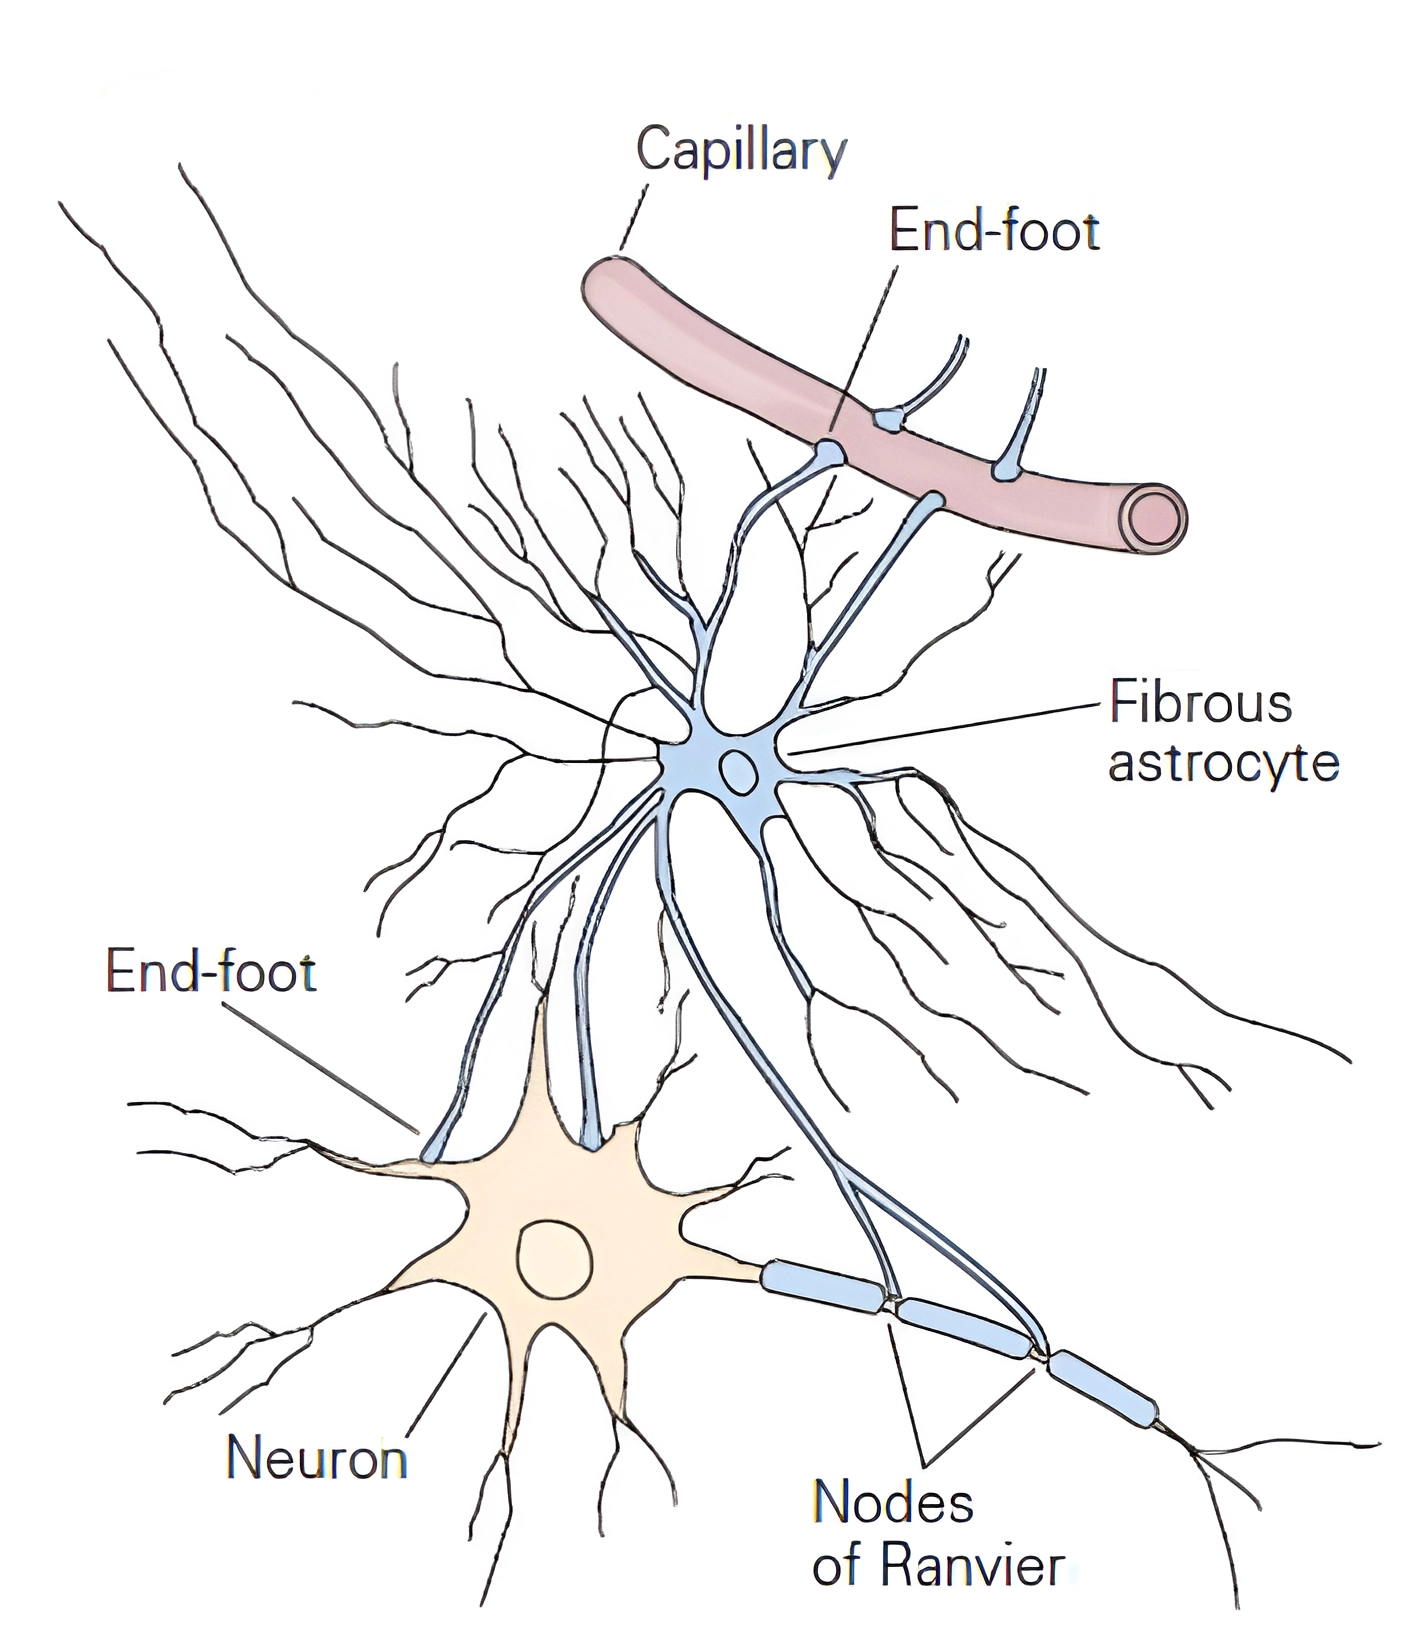
\includegraphics[width=\textwidth]{./img/astrocyte.png}
\end{minipage}\\[1em]

\begin{minipage}{0.79\textwidth}
    \begin{descriptionlist}
        \item[Oligodendrocytes and Schwann cells] \marginnote{Oligodendrocytes\\Schwann cells}
            Oligodendrocytes are located in the central nervous system, while 
            Schwann cells are located in the peripheral nervous system.
            \begin{itemize}
                \item Produce thin sheets of myelin that wrap concentrically around the axon of the neurons.
                    This insulating material allows the rapid conduction of electrical signals along the axon.
            \end{itemize}

            \begin{remark}
                Myelin is white, giving the name to the white matter.
            \end{remark}

            \begin{remark}
                In multiple sclerosis, the immune system attacks the oligodendrocytes, 
                slowing or disrupting messages traveling along the nerves.
            \end{remark}
    \end{descriptionlist}
\end{minipage}
\begin{minipage}{0.2\textwidth}
    \centering
    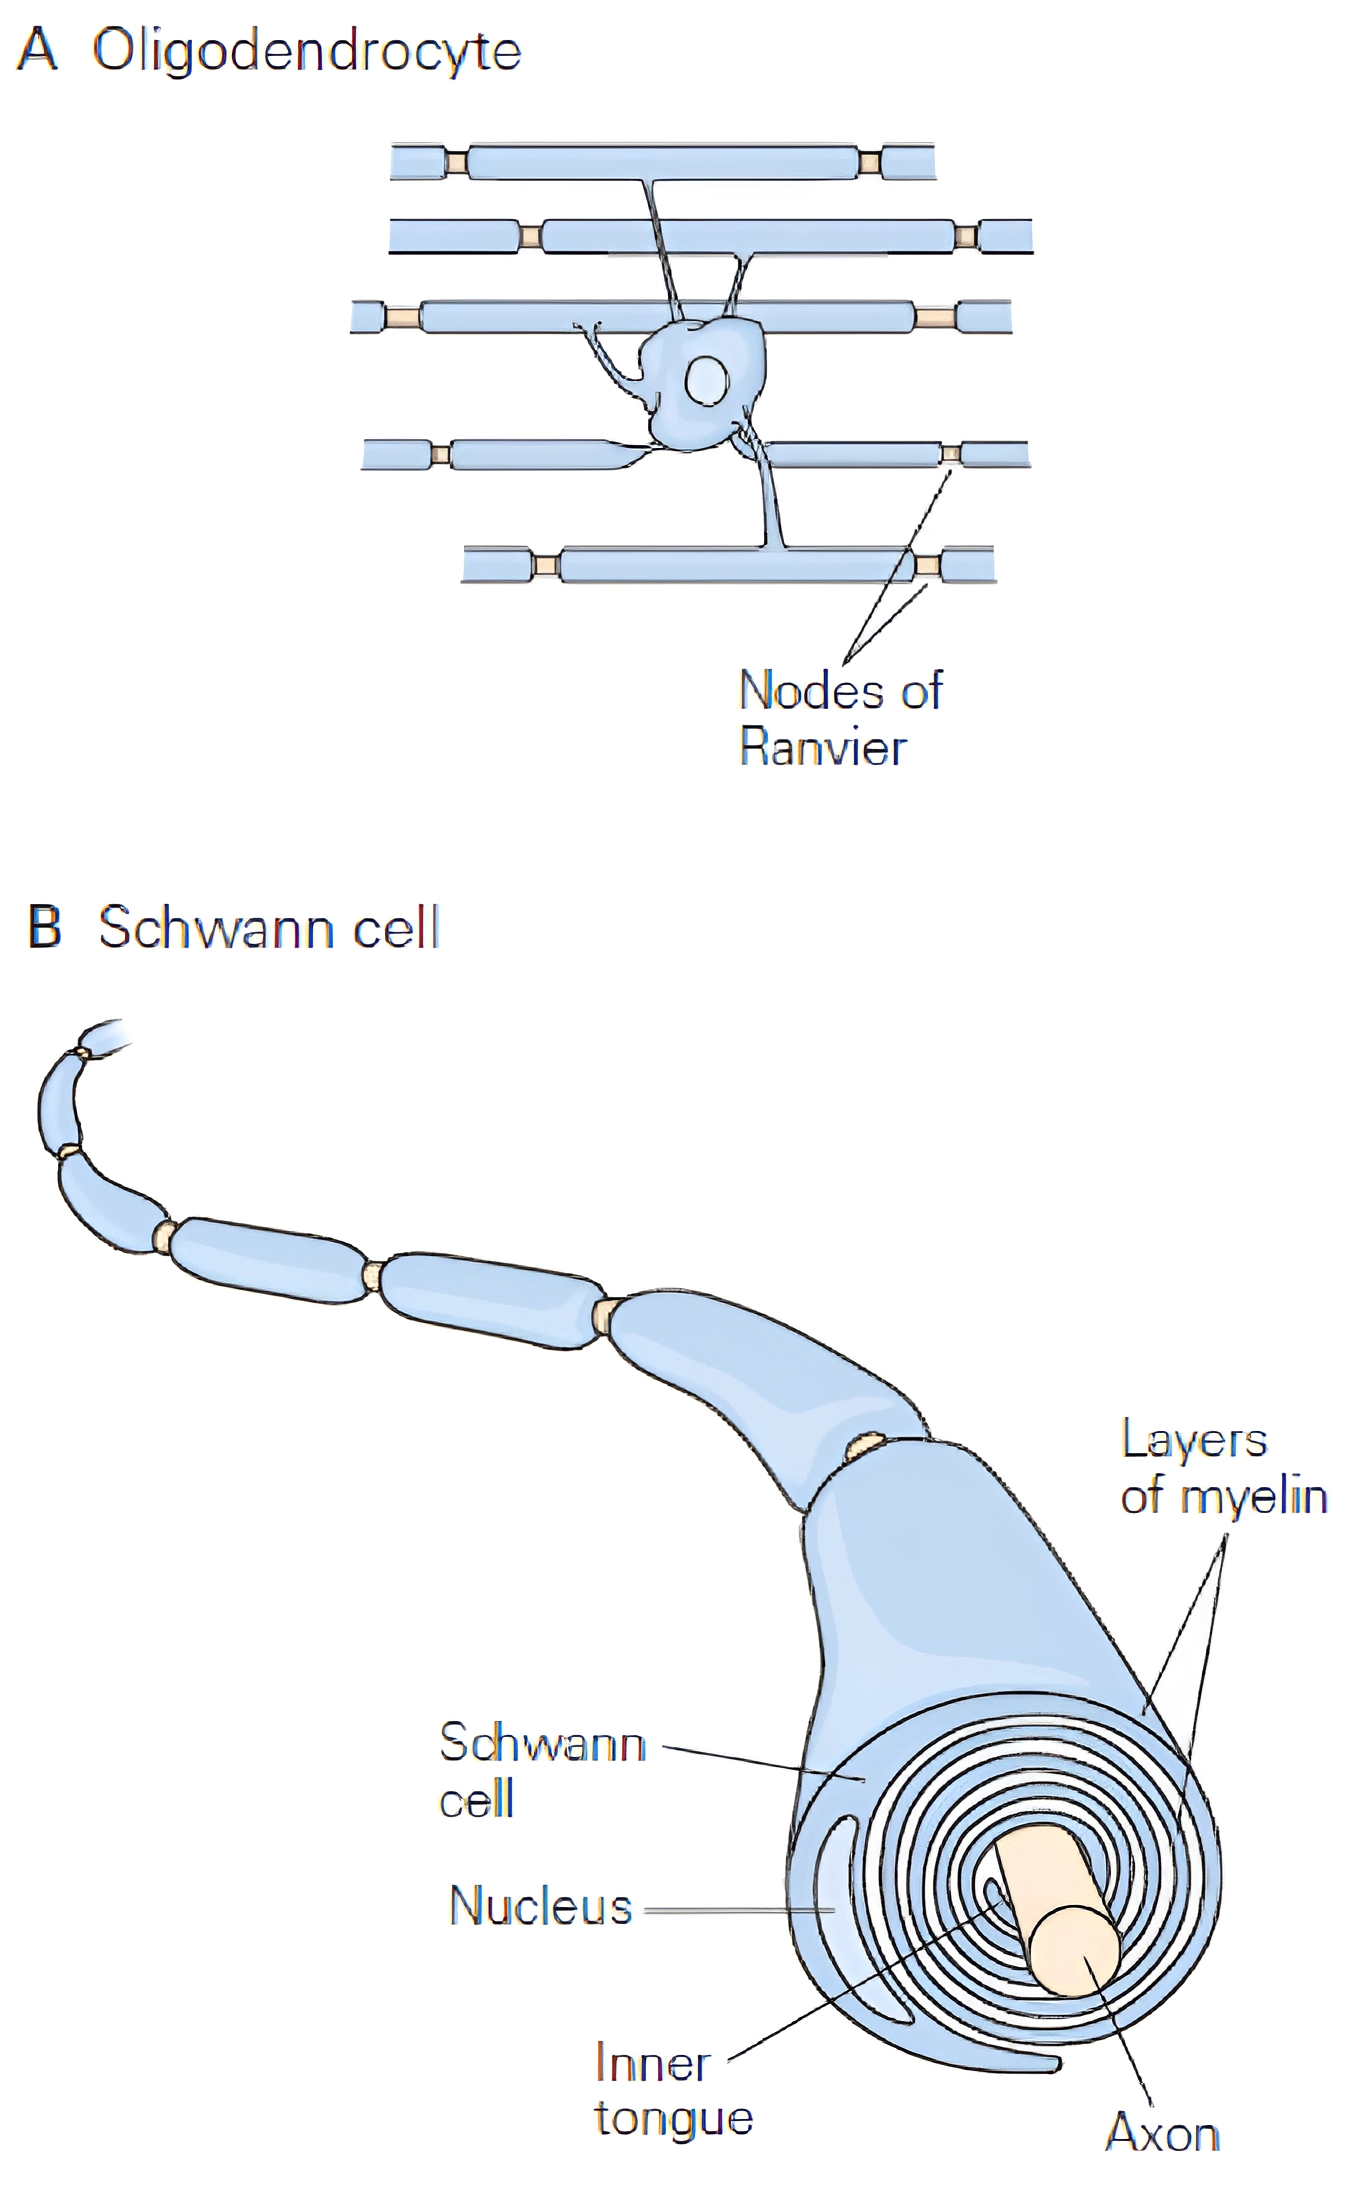
\includegraphics[width=\textwidth]{./img/insulation.png}
\end{minipage}



\subsection{Neurons / Nerve cells}
\marginnote{Neurons/Nerve cells}

A nervous system has around 100 billion neurons.
There are 100 distinct types of neurons varying in form, location, and interconnectivity.

Generally, a neuron does the following:
\begin{enumerate}
    \item Receives some information.
    \item Makes a decision.
    \item Passes it to other neurons.
\end{enumerate}

\begin{description}
    \item[Eukaryotic cell] \marginnote{Eukaryotic cell}
        A neuron is an eukaryotic cell. Therefore, it has:
        \begin{description}
            \item[Cell membrane] Membrane that separates the intracellular and extracellular space.
            \item[Cytoplasm] Intracellular fluid mainly made of proteins and ions of potassium, sodium, chloride, and calcium.
            \item[Extracellular fluid] Fluid in which the neuron sits. Similar composition of the cytoplasm.
            \item[Cell body/soma] Metabolic center of the cell.
        \end{description}

        \begin{figure}[h]
            \centering
            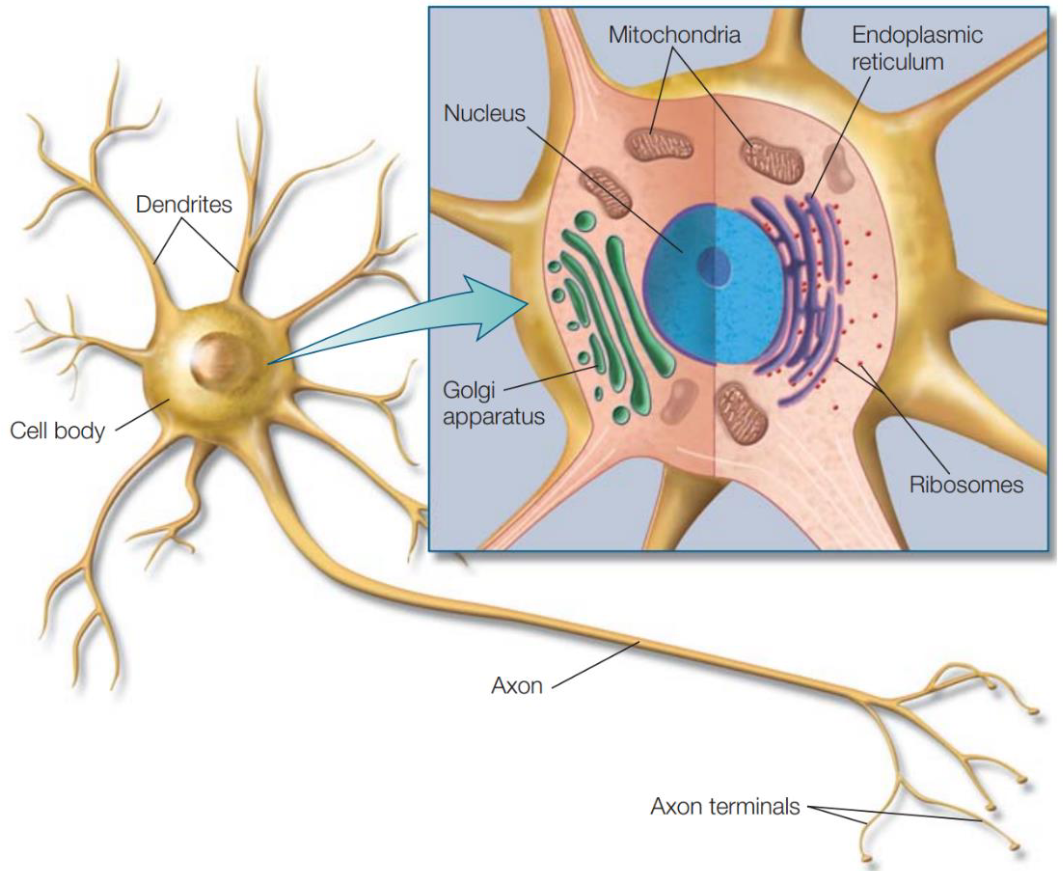
\includegraphics[width=0.5\textwidth]{img/neuron_eukaryotic.png}
            \caption{Neuron as an eukaryotic cell}
        \end{figure}
\end{description}

\begin{description}
    \item[Neuron-specific components] \phantom{}
        \begin{description}
            \item[Dendrites] \marginnote{Dendrites}
                Receives the outputs of other neurons.
                A neuron has multiple dendrites with different shapes depending on the type and location of the neuron.
            \item[Axon] \marginnote{Axon}
                Transmitting zone of the neuron that carries electrical signals from the dendrites to the synapses (from 0.1mm to 2m).
                A neuron has a single axon.
            \item[Synapses] \marginnote{Synapses}
                Represents the output zone of the neuron from where electrical or chemical signals can be transmitted to other cells.
                A neuron has multiple synapses.

                \begin{description}
                    \item[Presynaptic cell] Cell transmitting a signal.
                    \item[Postsynaptic cell] Cell receiving a signal.
                    \item[Synaptic cleft] Narrow space separating presynaptic and postsynaptic cells (i.e. the space separating two neurons).
                \end{description}
        \end{description}
\end{description}

\begin{figure}[H]
    \centering
    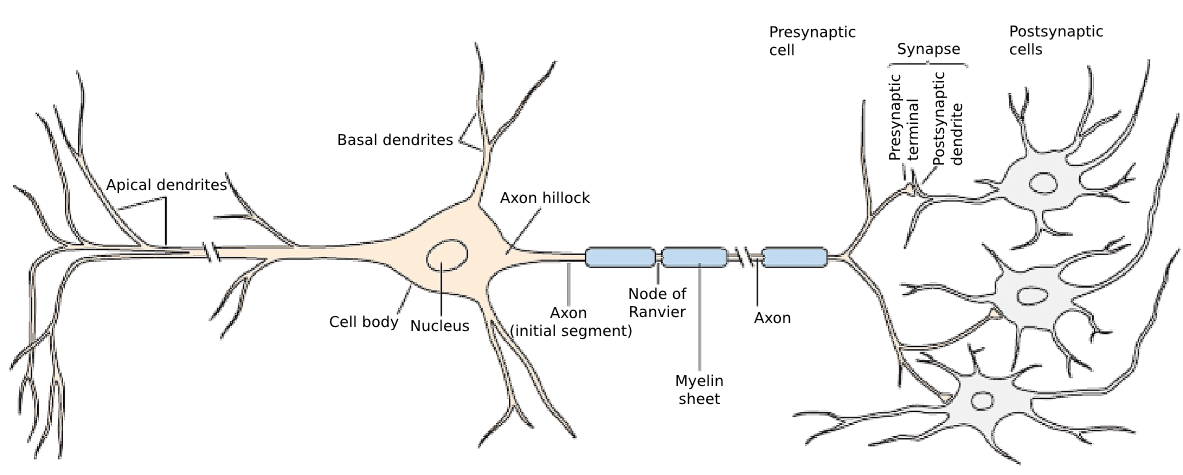
\includegraphics[width=0.9\textwidth]{img/neuron_specific.png}
    \caption{Neuron-specific components}
\end{figure}

There are three types of synapses:
\begin{descriptionlist}
    \item[Axosomatic] \marginnote{Axosomatic}
        Synapses that a neuron makes onto the cell body (soma) of another neuron.
    \item[Axodendritic] \marginnote{Axodendritic}
        Synapses that a neuron makes onto the dendrites of another neuron.
    \item[Axoaxonic] \marginnote{Axoaxonic}
        Synapses that a neuron makes onto the synapses of another neuron.
        In this case, the transmitting neuron can be seen as a signal modulator of the receiving neuron.
    \begin{figure}[h]
        \begin{subfigure}{.3\textwidth}
            \centering
            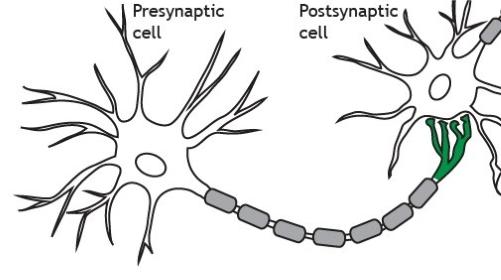
\includegraphics[width=\linewidth]{./img/axosomatic.png}
            \caption{Axosomatic}
        \end{subfigure}
        \begin{subfigure}{.3\textwidth}
            \centering
            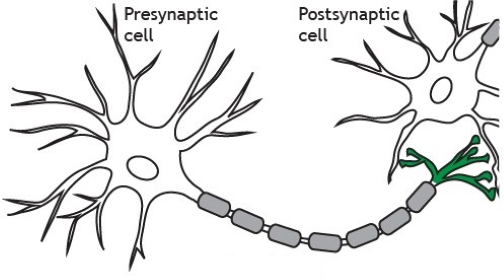
\includegraphics[width=\linewidth]{./img/axodendritic.png}
            \caption{Axodendritic}
        \end{subfigure}
        \begin{subfigure}{.3\textwidth}
            \centering
            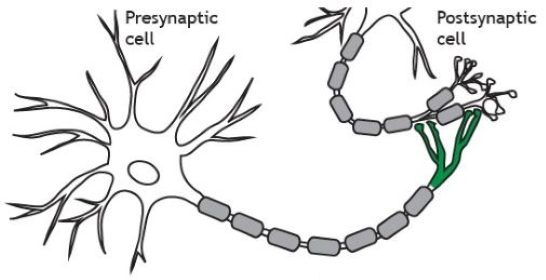
\includegraphics[width=\linewidth]{./img/axoaxonic.png}
            \caption{Axoaxonic}
        \end{subfigure}
    \end{figure}
\end{descriptionlist}

Neurons are divided into three functional categories:
\begin{descriptionlist}
    \item[Sensory neurons] \marginnote{Sensory neurons}
        Carry information from the body's peripheral sensors into the nervous system.
        Provides both perception and motor coordination.

    \item[Motor neurons] \marginnote{Motor neurons}
        Carry commands from the brain or the spinal cord to muscles and glands.

    \item[Interneurons] \marginnote{Interneurons}
        Intermediate neurons between sensory and motor neurons.
\end{descriptionlist}

\begin{description}
    \item[Principle of connectional specificity] \marginnote{Principle of connectional specificity}
        Neurons do not connect randomly but rather make specific connections at particular contact points.
\end{description}



\section{Information transfer within a neuron}


\subsection{Neuron functional regions}

In a neuron, there are four regions that handle signals:
\begin{descriptionlist}
    \item[Input zone] \marginnote{Input zone}
        Dendrites collect information from different sources
        in the form of \aclp{psp} (\acp{psp}).

    \item[Integration/trigger zone] \marginnote{Integration/trigger zone}
        \acp{psp} are summed at the axon hillock and an \ac{ap} is generated if a threshold (-55mV) has been exceeded.

    \item[Conductive zone] \marginnote{Conductive zone}
        The \ac{ap} is propagated through the axon.

    \item[Output zone] \marginnote{Output zone}
        Synapses transfer information to other cells.

        \begin{description}
            \item[Chemical synapses] The frequency of \acp{ap} determines the amount of neurotransmitters released.
            \item[Electrical synapses] The \ac{ap} is directly transmitted to the next neurons.
        \end{description}

    \begin{figure}[h]
        \centering
        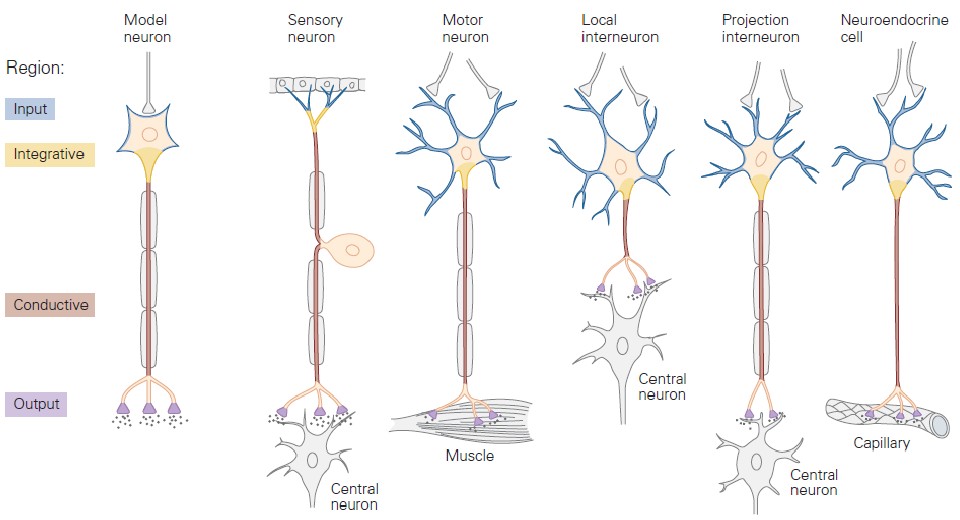
\includegraphics[width=0.8\textwidth]{./img/neuron_transmission.png}
        \caption{Transmitting regions of different types of neurons}
    \end{figure}

    \begin{figure}[h]
        \centering
        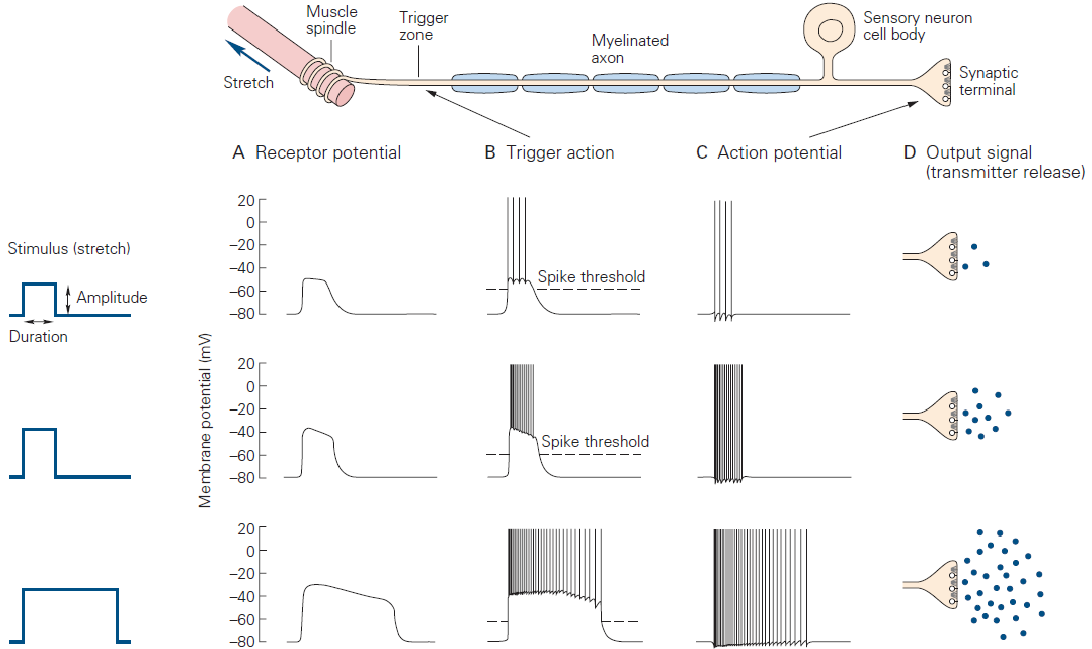
\includegraphics[width=0.8\textwidth]{./img/neuron_transmission2.png}
        \caption{Signal from the input to the output zones}
    \end{figure}
\end{descriptionlist}


\subsection{Neuron transmission signals}

\begin{description}
    \item[Resting membrane potential] \marginnote{Resting membrane potential}
        In a resting neuron, the voltage inside the cell is more negative ($-70$mV) than the outside.
        This allows the creation of an electrical signal when needed.

    \item[\Acl{psp} (\ac{psp})] \marginnote{\Acl{psp} (\ac{psp})}
        Small change in the membrane potential that alters the resting voltage of the cell.
        
        A \ac{psp} can be:
        \begin{descriptionlist}
            \item[Excitatory \ac{psp} (\acs{epsp})] \marginnote{Excitatory \ac{psp}}
                Has a depolarizing role: produces a decrease in the membrane potential (i.e. increases voltage inside the cell), 
                therefore enhancing the ability to generate an \ac{ap}.

            \item[Inhibitory \ac{psp} (\acs{ipsp})] \marginnote{Inhibitory \ac{psp}}
                Has a hyperpolarizing role: produces an increase in the membrane potential (i.e. reduces voltage inside the cell), 
                therefore reducing the ability to generate an \ac{ap}.
        \end{descriptionlist}

        A \ac{psp} has the following properties:
        \begin{itemize}
            \item The amplitude and duration of the signal are determined by the size of the stimulus that caused it.
                Overall, the amplitude is small.
            \item The signal is passively conducted through the cytoplasm, therefore it decays with distance and is able to travel 1mm at most.
            \item A single \acs{epsp} is not enough to fire a neuron. Multiple \acp{psp} are summed at the axon hillock.
                There are two types of summation:
                \begin{descriptionlist}
                    \item[Spatial summation] Sum of the \acp{psp} received at the same time.
                    \item[Temporal summation] Sum of the \acp{psp} received at different time points.
                \end{descriptionlist}

                \begin{remark}
                    The fact that a single \ac{epsp} is not enough to fire a neuron prevents a response to every single stimulus.
                \end{remark}
        \end{itemize}

    \item[\Acl{ap} (\ac{ap})] \marginnote{\Acl{ap} (\ac{ap})}
        Signal generated when the sum of \acp{epsp} exceeds a fixed threshold of $-55$mV (all-or-none).

        \begin{description}
            \item[Saltatory conduction] \marginnote{Saltatory conduction}
                Mechanism that allows a fast propagation on long distances of \acp{ap}.
                \begin{enumerate}
                    \item Depolarization causes the sodium ion (Na+) channels located in the nodes of Ranvier of the axon to gradually open.
                    \item Na+ flows into the neuron and further depolarizes it until the Na+ equilibrium potential is reached.
                    \item With Na+ equilibrium, Na+ channels close and potassium ion (K+) channels open.
                    \item K+ flows into the neuron and restores the membrane potential until the K+ equilibrium potential is reached.
                    \item With K+ equilibrium, K+ channels close and 
                        the membrane potential of the neuron is more negative than the resting potential (hyperpolarization).
                        It will gradually return to its resting potential.
                        \begin{remark}
                            During hyperpolarization, Na+ channels cannot open (refractory period).
                            This has two implications:
                            \begin{itemize}
                                \item It limits the number of times a neuron can fire in a given time.
                                \item Guarantees a unidirectional electrical current flow 
                                    (\textbf{Principle of dynamic polarization}).\marginnote{Principle of dynamic polarization} 
                            \end{itemize}
                        \end{remark}
                \end{enumerate}

                \begin{figure}[H]
                    \begin{subfigure}{.45\textwidth}
                        \centering
                        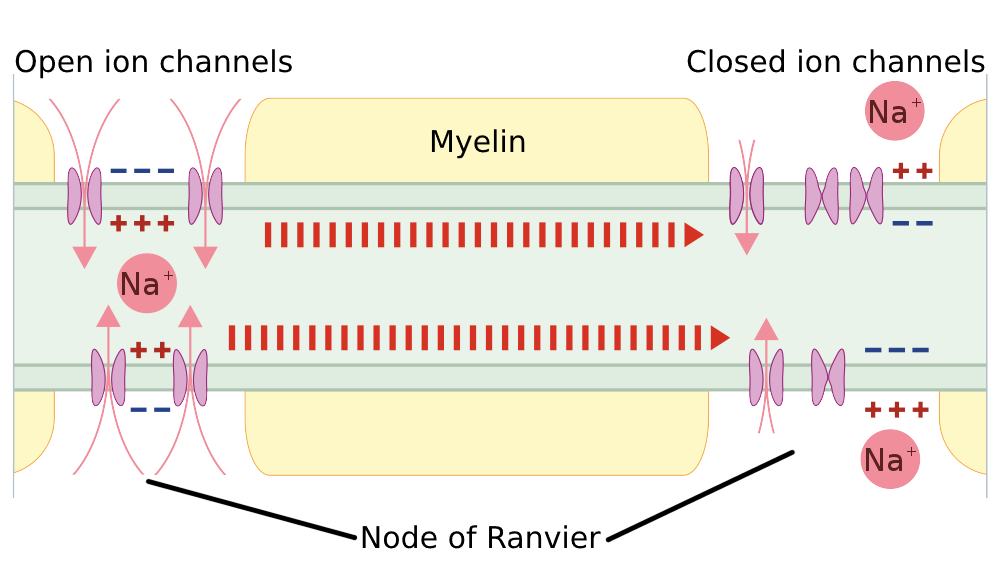
\includegraphics[width=0.85\textwidth]{./img/saltatory_conduction.png}
                        \caption{Ion channels along the axon}
                    \end{subfigure}
                    \begin{subfigure}{.45\textwidth}
                        \centering
                        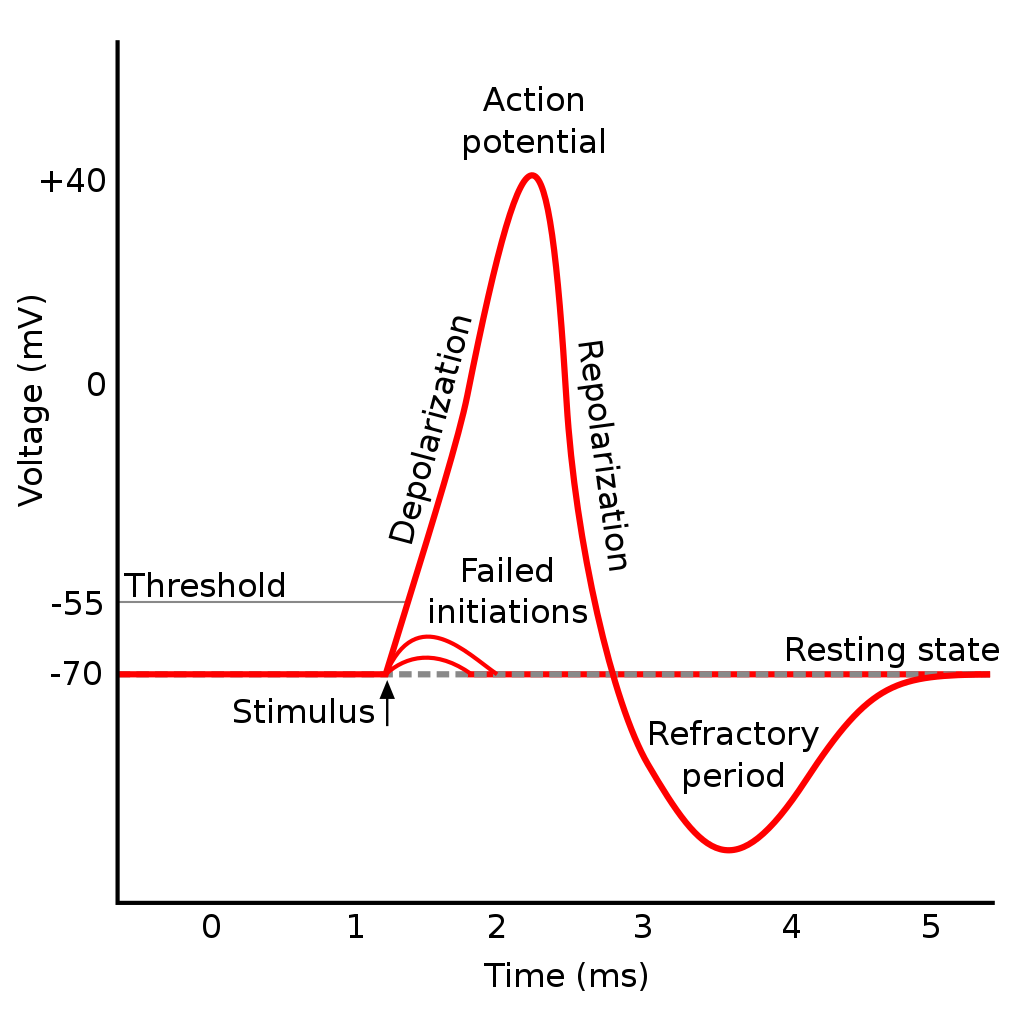
\includegraphics[width=0.8\textwidth]{./img/action_potential.png}
                        \caption{Triggering of an action potential}
                    \end{subfigure}
                \end{figure}
        \end{description}


        \begin{remark}
            As the signal is constantly regenerated, 
            \Acp{ap} have similar amplitude and duration in all neurons, regardless of the characteristics of the input \acp{psp}.
            Therefore, the only way an \ac{ap} has to carry information is by varying frequency and firing duration, making it a binary signal.
        \end{remark}
\end{description}

\begin{example}
    Seizures are caused by misfiring neurons.
\end{example}



\section{Information transfer between two neurons}


\subsection{Electrical synapse}

\begin{minipage}{0.55\textwidth}
    \begin{description}
        \item[Structure] \marginnote{Electrical synapse}
            The neuronal membranes of the presynaptic and postsynaptic neurons are in contact at \textbf{gap junctions} and
            the cytoplasm of the two neurons is virtually continuous through connecting \textbf{pores}.
    \end{description}
\end{minipage}
\begin{minipage}{0.35\textwidth}
    \centering
    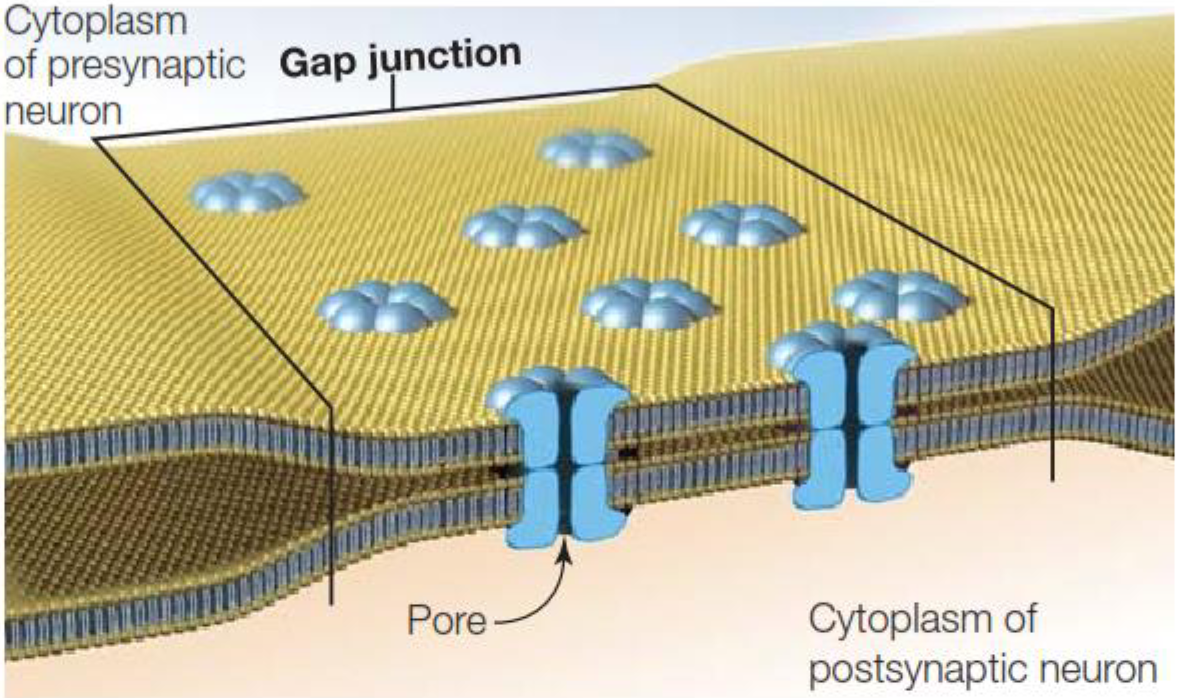
\includegraphics[width=\linewidth]{./img/electric_synapse.png}
\end{minipage}

\begin{description}
    \item[Functioning]
        The two neurons are \textbf{isopotential} (i.e. they have the same membrane potential) and 
        the ions of the presynaptic neurons are instantaneously transmitted to the postsynaptic neuron.

    \item[Properties] \phantom{}
        \begin{itemize}
            \item Fast transmission.
            \item Allows for synchronous operations involving groups of neurons.
            \item The strength of the signal cannot be modulated.
        \end{itemize}
\end{description}


\subsection{Chemical synapse}

\begin{description}
    \item[Structure] \marginnote{Chemical synapse}
        The synaptic cleft separates the presynaptic and postsynaptic neurons.
        \begin{description}
            \item[Neurotransmitter] 
                Chemical substance received by the receptors of the postsynaptic neuron.

                The effect of a neurotransmitter is decided by the receiving receptor and not by the cell transmitting it.

            \item[Presynaptic terminals] 
                Swellings at the end of the axon that contain synaptic vesicles.

            \item[Synaptic vesicles] 
                Vesicles containing neurotransmitter molecules.
        \end{description}

    \item[Functioning] 
        The release of neurotransmitter molecules is based on the following steps:
        \begin{enumerate}
            \item An action potential arriving at the terminal of a presynaptic axon causes the calcium ion (Ca$^{2+}$) voltage-gates to open.
            \item Ca$^{2+}$ flow into the cell and 
                cause the synaptic vesicles to bind to the cell membrane to release neurotransmitters into the synaptic cleft.
            \item Neurotransmitters cross the synaptic cleft and bind to the receptors of the postsynaptic neuron.
                Depending on the neurotransmitter and the receiving receptor, there might be a generation of \ac{epsp} or \ac{ipsp}.
        \end{enumerate}

        \begin{center}
            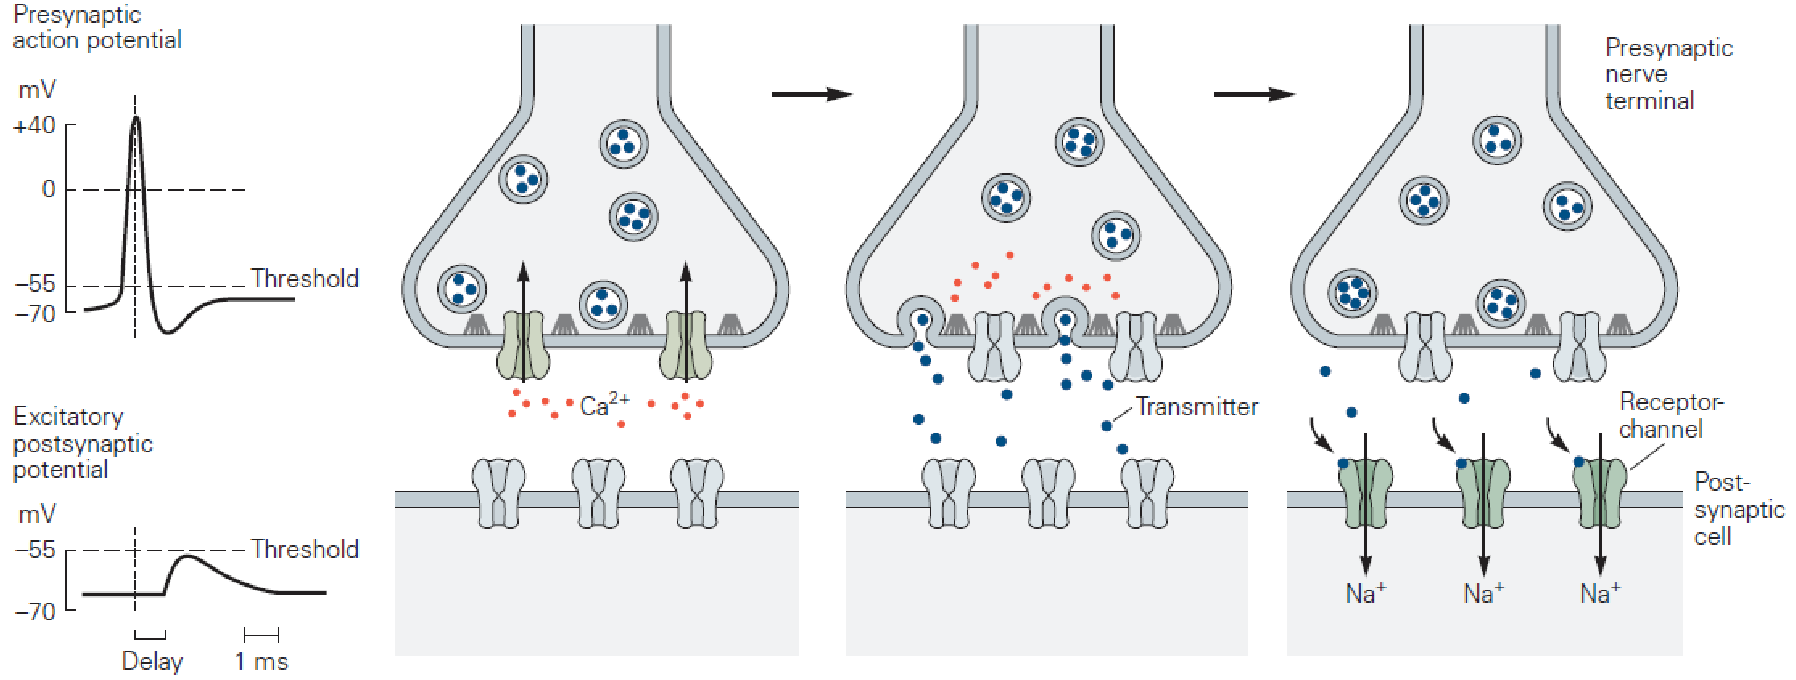
\includegraphics[width=0.9\linewidth]{./img/chemical_synapse.png}
        \end{center}

        When a receptor recognizes the neurotransmitter, it is released back into the synaptic cleft.
        To avoid a constant stimulation of the receptors, neurotransmitters are inactivated:
        \begin{itemize}
            \item The synaptic terminal can reuptake neurotransmitters through transporter proteins.
            \item Neurotransmitters might degenerate or be broken down by special enzymes.
            \item Neurotransmitters can be released far away from the site of the receptors.
        \end{itemize}

    \item[Properties] \phantom{}
        \begin{itemize}
            \item Slow transmission.
            \item The signal can be modulated.
            \item Has specific effects depending on the neurotransmitter and the receptors.
        \end{itemize}
\end{description}



\section{Neural circuit}

\begin{description}
    \item[Neural circuit] \marginnote{Neural circuit}
        Group of interconnected neurons that process a specific kind of information.

        \begin{remark}
            The behavioral function of each neuron is determined by its connections.
        \end{remark}

    \item[Types of neurons] \phantom{}
        \begin{description}
            \item[Sensory neuron] \marginnote{Sensory neuron}
                Carry information from the peripheral sensors to the nervous system for both perception and motor coordination.
        
            \item[Motor neuron] \marginnote{Motor neuron}
                Carry information from the nervous system to muscles and glands.
            
            \item[Interneuron] \marginnote{Interneuron}
                Intermediate neurons between sensory and motor neurons.
        \end{description}
\end{description}

\begin{remark}
    In vertebrates, a stimulus causes multiple neural pathways to simultaneously encode different information.
    This allows for parallel processing to increase both the speed and reliability of the information transfer.
\end{remark}

\begin{description}
    \item[Neural pathways types] \phantom{}
        \begin{description}
            \item[Divergent pathway] \marginnote{Divergent pathway}
                One neuron activates many target cells.
                Typically happens at the input stages of the nervous system
                to ensure that a single neuron has a wide and diverse influence.

            \item[Convergent pathway] \marginnote{Convergent pathway}
                Many neurons activate a single target cell.
                Typically happens at the output stages of the nervous system 
                to ensure that a motor neuron is activated only when a sufficient number of neurons are firing.
        \end{description}

    \item[Neuron firing types] \phantom{}
        \begin{description}
            \item[Excitatory neuron] \marginnote{Excitatory neuron}
                Neurons that produce signals that increase the probability of firing of the postsynaptic neurons.
                
            \item[Inhibitory neuron] \marginnote{Inhibitory neuron}
                Neurons that produce signals that decrease the probability of firing of the postsynaptic neurons.
                
                \begin{description}
                    \item[Feed-forward inhibition] 
                        Excitatory neurons connected to inhibitory interneurons to block other downstream neurons.
                        Allows to enhance the active pathway and to block other antagonist actions.
                        \begin{figure}[H]
                            \centering
                            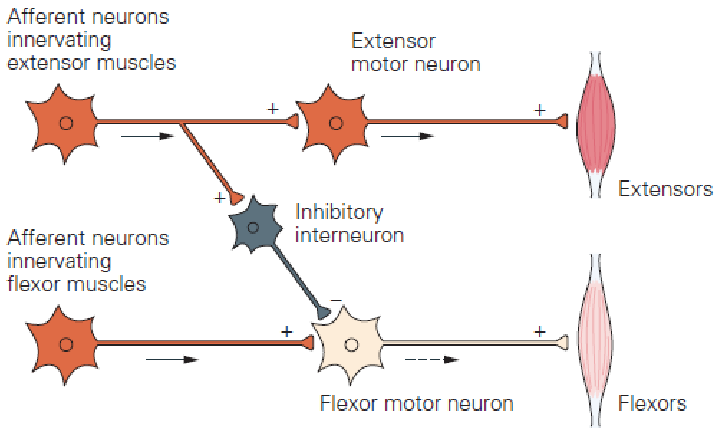
\includegraphics[width=0.4\textwidth]{./img/feedforward_inhibition.png}
                            \caption{Example of feed-forward inhibition}
                        \end{figure}

                    \item[Feed-back inhibition] 
                        Excitatory neurons connected to inhibitory interneurons that return to the same neurons to inhibit them.
                        Prevents the overload of neurons or muscles.
                        \begin{figure}[H]
                            \centering
                            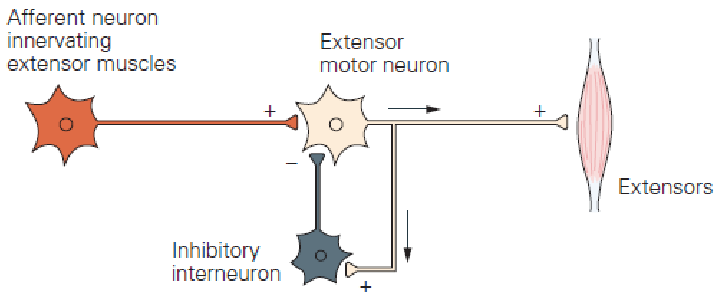
\includegraphics[width=0.4\textwidth]{./img/feedback_inhibition.png}
                            \caption{Example of feed-back inhibition}
                        \end{figure}
                \end{description}
        \end{description}
\end{description}



\begin{casestudy}[Knee-jerk reflex]
    By tapping the patellar tendon (below the kneecap), the following happens:
    \begin{enumerate}
        \item The sensory information is conveyed from the muscle to the spinal cord (central nervous system).
        \item The nervous system issues motor commands to the muscles which results in the knee jerk.
        \item Inhibitory commands are issued to stop antagonist muscles.
    \end{enumerate}

    \begin{center}
        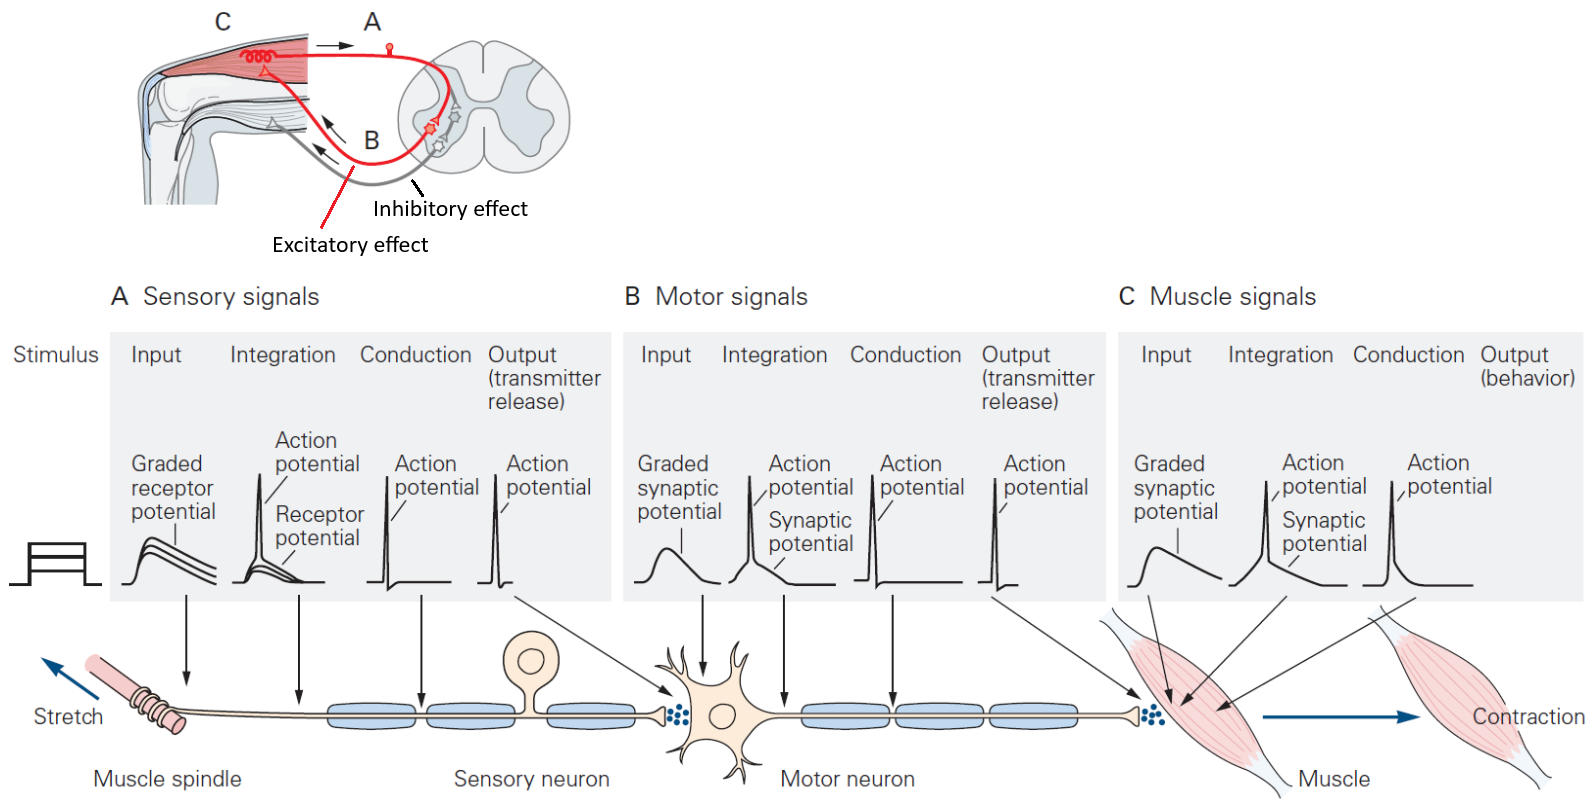
\includegraphics[width=0.8\textwidth]{./img/knee_jerk.png}
    \end{center}
\end{casestudy}


\section{Neural system}

\begin{figure}[H]
    \centering
    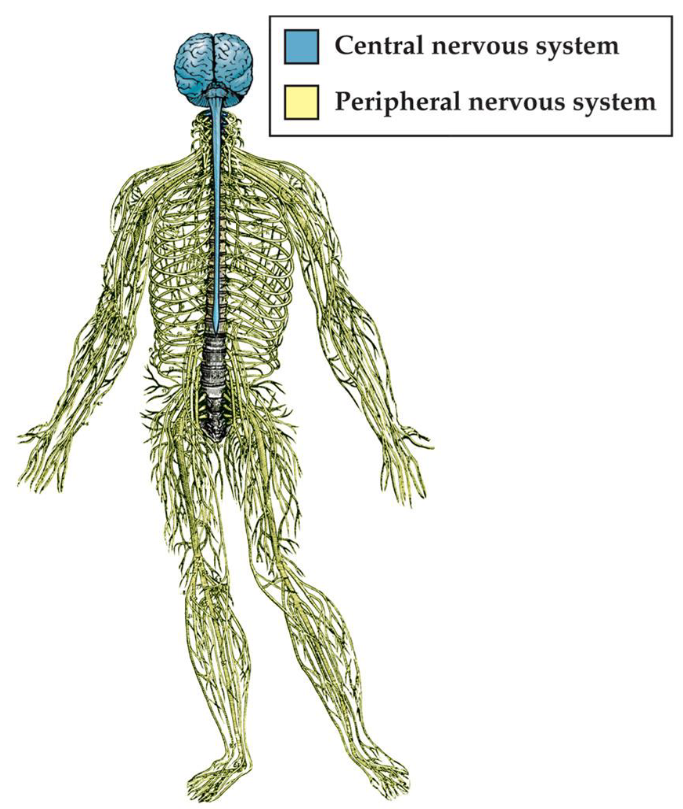
\includegraphics[width=0.3\textwidth]{./img/neural_system.png}
    \caption{Composition of the nervous system}
\end{figure}


\subsection{\Acl{pns} (\acs{pns})}

The \acl{pns} is composed of:
\begin{descriptionlist}
    \item[Nerves] \marginnote{Nerves}
        Groups of axons and glia.

    \item[Ganglia] \marginnote{Ganglia}
        Groups of neuron bodies outside the \acl{cns}
\end{descriptionlist}

The \ac{pns} has the following functions:
\begin{itemize}
    \item Delivers sensory information to the \acl{cns}.
    \item Carries commands from the \acl{cns} to the muscles.
    \item Supplies the \acl{cns} with information regarding both the external and internal environment.
\end{itemize}

The \ac{pns} has the following divisions:
\begin{descriptionlist}
    \item[Somatic nervous system] \marginnote{Somatic nervous system} \phantom{}
        \begin{itemize}
            \item Sensory neurons that receive information from the skin, muscles, and joints.
            \item Converts perceived spatial and physical information into electrical signals for the \acl{cns} to process.
            \item Controls the voluntary muscles.
        \end{itemize}

    \item[Autonomic nervous system] \marginnote{Autonomic nervous system} \phantom{}
        \begin{itemize}
            \item Controls internal organs (viscera), the vascular system, and involuntary muscles and glands.
            \item Divided into three systems:
                \begin{descriptionlist}
                    \item[Sympathetic system] \marginnote{Sympathetic system}
                        Operates antagonistically against the parasympathetic system.
                        Handles the body's response to stress (using norepinephrine).

                        Physically, the sympathetic system originates from the spinal cord. 
                        Its ganglia are closer to the spinal cord,
                        therefore the axons from the \acl{cns} to the ganglia are shorter than the axons from the ganglia to the organs.

                        \begin{example}
                            Stimulates adrenal glands to prepare the body for action (fight or flight),
                            increases heart rate,
                            diverts the blood from the digestive tract to the somatic musculature, \dots
                        \end{example}

                    \item[Parasympathetic system] \marginnote{Parasympathetic system}
                        Operates antagonistically against the sympathetic system.
                        Acts to preserve the body's resources and restore homeostasis (using acetylcholine).

                        Physically, the parasympathetic system originates from the base of the brain and from the sacral spinal cord.
                        Its ganglia are outside the spinal cord, sometimes inside the affected organs,
                        therefore the axons from the \acl{cns} to the ganglia are longer than the axons from the ganglia to the organs.

                        \begin{example}
                            Slows heart rate, stimulates digestion, \dots
                        \end{example}

                    \item[Enteric system] \marginnote{Enteric system}
                        Controls the involuntary muscles of the gut.
                \end{descriptionlist}
        \end{itemize}
\end{descriptionlist}



\subsection{\Acl{cns} (\acs{cns})}

\begin{description}
    \item[Meninges] \marginnote{Meninges}
        Three layers of membrane protecting the brain and the spinal cord.
        \begin{descriptionlist}
            \item[Dura mater] The outermost and thickest layer.
            \item[Arachnoid mater] The middle layer.
            \item[Pia mater] The innermost and most delicate layer. It adheres to the brain's surface.
        \end{descriptionlist}

    \item[Cerebrospinal fluid] \marginnote{Cerebrospinal fluid}
        Fluid that allows the brain to float and prevents it from simply sitting on the skull surface.
        It also reduces the shock to the brain and the spinal cord in case of rapid accelerations/decelerations.

        The fluid is located in:
        \begin{itemize}
            \item The space between the arachnoid mater and the pia mater.
            \item The brain ventricles.
            \item Cisterns and sulcis.
            \item The central canal of the spinal cord.
        \end{itemize}

    \item[Blood-brain barrier] \marginnote{Blood-brain barrier}
        Barrier between the brain's capillaries and the brain's tissue.
        It protects against pathogens and toxins.

        \begin{remark}
            The effectiveness of the barrier also prevents drugs to treat mental and neurological disorders from passing through.
        \end{remark}

    \item[Spinal cord] \marginnote{Spinal cord}
        Acts as a relay for the information coming in and out of the brain.
        It is enclosed in the vertebral column.
\end{description}

\begin{remark}
    Most pathways in the \ac{cns} are bilaterally symmetrical: 
    the sensory and motor activities of one side of the body are handled by the cerebral hemisphere on the opposite side.
\end{remark}

\begin{description}
    \item[Brain] \marginnote{Brain}
    
    \begin{minipage}{0.6\textwidth}
        \begin{description}
            \item[Brain stem] \marginnote{Brain stem}
                Regulates basic life functions such as blood pressure, respiration, and sleep/wakefulness.
                It is divided into three sections:
                \begin{itemize}
                    \item Medulla.
                    \item Pons.
                    \item Midbrain.
                \end{itemize}
        \end{description}
    \end{minipage}
    \begin{minipage}{0.35\textwidth}
        \centering
        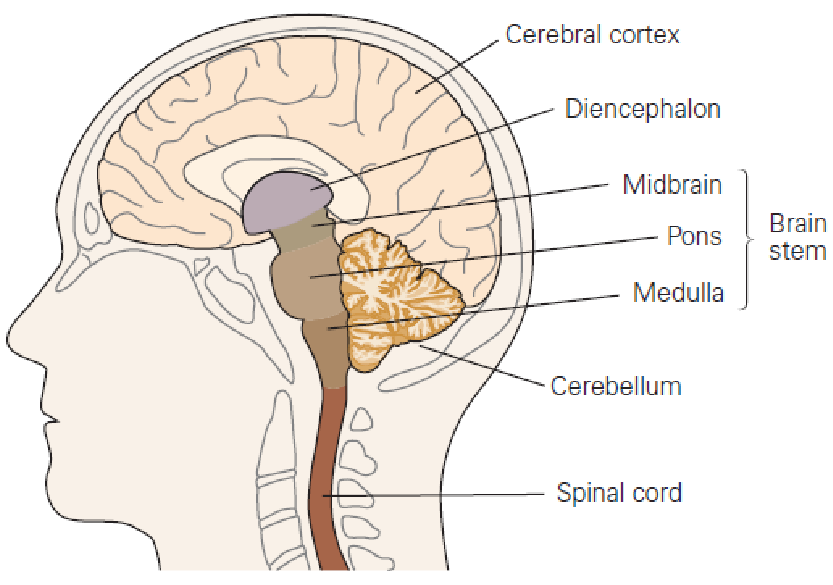
\includegraphics[width=\linewidth]{./img/brain_sections.png}
    \end{minipage}

    \begin{description}
        \item[Cerebellum] \marginnote{Cerebellum}
            Contains lots of neurons and is responsible for:
            \begin{itemize}
                \item Maintaining posture.
                \item Coordinating head, eye, and arm movement.
                \item Regulating motor control (i.e. adjustments to the movement).
                \item Learning motor skills.
            \end{itemize}

        \item[Diencephalon] \marginnote{Diencephalon} 
            \phantom{}\\
            \begin{minipage}{0.6\linewidth}
                \begin{description}
                    \item[Thalamus] \marginnote{Thalamus}
                        Sorts incoming sensory information (except the sense of smell) of the \acl{pns} and 
                        sends them to the sensory regions of the cerebral hemispheres.
                    \item[Hypothalamus] \marginnote{Hypothalamus}
                        Regulates the autonomic nervous system and homeostasis through the pituitary gland (which releases hormones).
                        Handles the motivation system of the brain by favoring behaviors the organism finds rewarding.
                \end{description}
            \end{minipage}
            \begin{minipage}{0.35\linewidth}
                \centering
                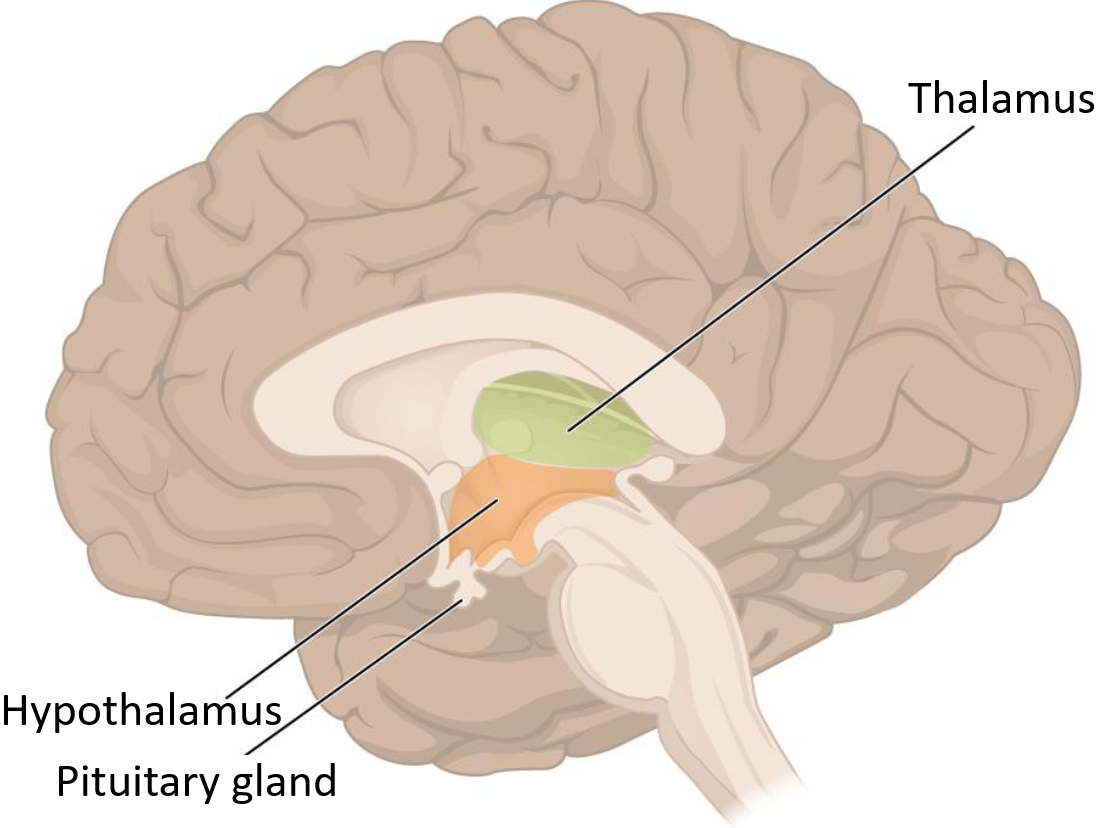
\includegraphics[width=\linewidth]{./img/diencephalon.png}
            \end{minipage}

        \item[Telencephalon/Cerebral hemispheres] \marginnote{Telencephalon/Cerebral hemispheres}
            Consists of:
            \begin{description}
                \item[Cerebral cortex] 
                    Made of gray matter (body of neurons).

                \item[White matter] 
                    (axons and glial cells).

                \item[Basal ganglia] \marginnote{Basal ganglia}
                    Receive inputs from sensory and motor areas and 
                    mostly send them through the thalamus to the frontal lobe.

                    They have a crucial role in motor control and reinforcement learning.
                    This happens through two pathways:
                    \begin{descriptionlist}
                        \item[Direct pathway] When active, it causes the disinhibition of the thalamus and has the consequence of initializing movement.
                        \item[Indirect pathway] When active, it causes the inhibition of the thalamus and consequently inhibits movement.
                    \end{descriptionlist}
                    To activate the direct pathway and inhibit the indirect pathway, the substantia nigra pars compacta (SNc) releases the neurotransmitter dopamine.

                    \begin{example}[Parkinson's disease]
                        In patients affected by Parkinson's disease, the dopamine-related neurons in the SNc are lost causing
                        an overactivation of the indirect pathway that inhibits movement.
                    \end{example}

                \item[Amygdala] \marginnote{Amygdala}
                    Responsible for recognizing a stimulus and reacting to it.
                    Involved in attention, perception, value representation, decision-making, learning, memory, \dots

                \item[Hippocampus] \marginnote{Hippocampus}
                    Responsible for long-term memory and spatial memory.
            \end{description}

        \item[Cerebral cortex] \marginnote{Cerebral cortex}
            Surface of the brain which covers around 2.2m$^2$ to 2.4m$^2$.
            To cover more surface, the cortex has infoldings (sulci and gyri) which also allow to connect neurons with shorter axons.

            There are two symmetrical hemispheres connected through the corpus callosum and four different lobes.

            \begin{figure}[H]
                \centering
                \begin{subfigure}{0.25\linewidth}
                    \centering
                    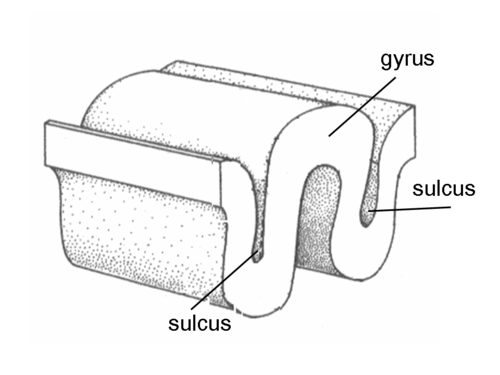
\includegraphics[width=\linewidth]{./img/brain_surface.png}
                    \caption{Visualization of sulci and gyri}
                \end{subfigure}
                \begin{subfigure}{0.35\linewidth}
                    \centering
                    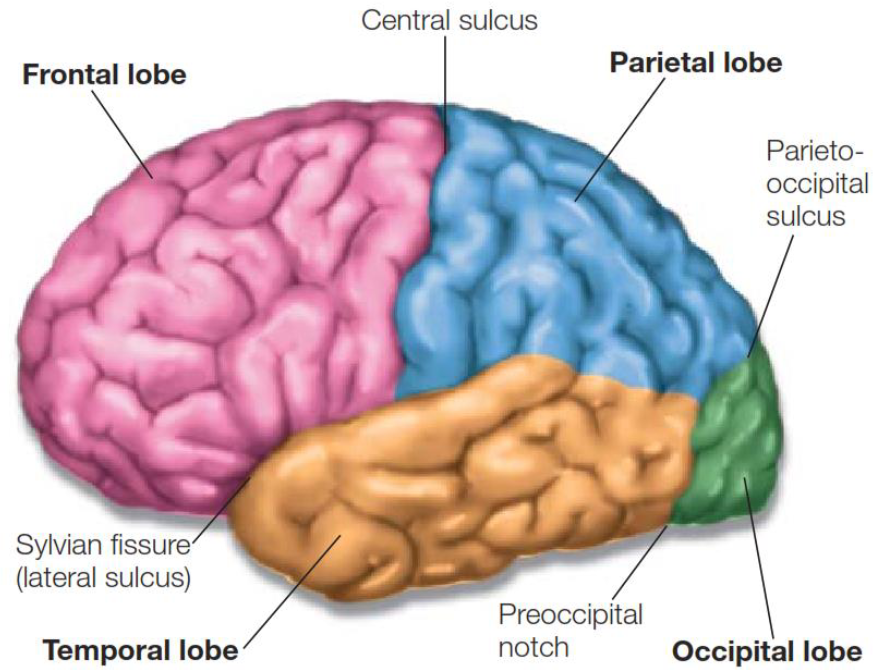
\includegraphics[width=\linewidth]{./img/brain_lobes.png}
                    \caption{Lobes of the brain}
                \end{subfigure}
            \end{figure}

            \begin{description}
                \item[Frontal lobe] \marginnote{Frontal lobe}
                    \phantom{}
                    \begin{description}
                        \item[Motor cortex] \phantom{}
                            \begin{itemize}
                                \item Planning and execution of movement.
                                \item Contains neurons that directly activate somatic movement neurons in the spinal cord.
                            \end{itemize}

                        \item[Prefrontal cortex] \phantom{}
                            \begin{itemize}
                                \item Long-term planning.
                                \item Decision making.
                                \item Motivation and value.
                            \end{itemize}
                    \end{description}
                

                \item[Parietal lobe] \marginnote{Parietal lobe}
                    Receives and integrates information from the outside world, the body, and memory.

                    \begin{description}
                        \item[Somatosensory cortex]
                            Receives information regarding touch, pain, temperature, and limb position.
                    \end{description}

                    \begin{remark}
                        Neurons responsible for a specific part of the body are clustered together.
                    \end{remark}


                \item[Occipital lobe] \marginnote{Occipital lobe}
                    \begin{description}
                        \item[Visual cortex] 
                            Responsible for vision. 
                            Encodes features like luminance, spatial frequency, orientation, motion, \dots
                    \end{description}

                    \begin{remark}
                        Neurons responsible for processing a specific feature are clustered together.
                    \end{remark}


                \item[Temporal lobe] \marginnote{Temporal lobe}
                    \begin{description}
                        \item[Auditory cortex]
                            Responsible for processing sound.
                    \end{description}

                    \begin{remark}
                        Neurons responsible for processing a specific sound frequency are clustered together.
                    \end{remark}

                \item[Association cortex] \marginnote{Association cortex}
                    Portion of the cortex that has neither sensory nor motor responsibility.
                    Receives and integrates inputs from many cortical areas.

                    \begin{description}
                        \item[Multisensory neuron]
                            Cell activated by multiple sensory modalities.
                    \end{description}
            \end{description}
    \end{description}
\end{description}